\chapter{User Experience}
\label{cap:user-experience}

Il redesign dell'interfaccia di un prodotto digitale richiede un'approfondita comprensione delle esigenze degli utenti, delle attività che devono svolgere e delle interazioni tra le varie componenti del sistema. Per raggiungere questo obiettivo, ho adottato un approccio integrato che combina il Design Centrato sull'Utente, il Design Centrato sull'Attività e il Design dei Sistemi, di cui parlerò nel capitolo \ref{cap:sviluppo-software}. Questo metodo mi ha permesso di disegnare e successivamente sviluppare un'interfaccia intuitiva, efficiente e capace di rispondere alle aspettative degli utenti finali.

\section{Design Centrato sull'Utente}

Il Design Centrato sull'Utente (User-Centered Design, UCD) è stato il punto di partenza fondamentale per il mio lavoro. La comprensione del target di utenti ha guidato ogni decisione progettuale, assicurando che l'interfaccia fosse realmente adatta a chi l'avrebbe utilizzata.\\

Il processo di User Experience è partito con una intervista ai vari stakeholder: qui ho compreso quali fossero gli obiettivi del prodotto iniziale e quali potessero essere le necessità evolutive.\\
Successivamente mi sono informata per comprendere chi fossero gli utenti del mio prodotto e capire meglio le loro necessità e aspettative. Le personas hanno rivelato informazioni cruciali:
\begin{itemize}
    \item necessità di accesso rapido alle informazioni: gli utenti hanno bisogno di trovare le informazioni immediatamente e in modo chiaro, senza dover navigare attraverso complicati menu.
    \item preferenza per la semplicità: il target desidera un'interfaccia pulita e semplice, priva di elementi superflui che potessero distrarre o confondere.
    \item efficacia ed efficienza: gli utenti sono persone spesso di fretta e non vogliono perdere tempo. Era essenziale che l'interfaccia consentisse di completare le operazioni rapidamente e senza intoppi.
\end{itemize}

\noindent Con queste informazioni ridisegnato l'interfaccia con un focus sulla chiarezza e l'usabilità, avvalendomi dell'utilizzo di mockup e wireframe. Per usabilità s'intende il grado con cui un prodotto può essere usato da determinati  utenti per raggiungere determinati obiettivi con efficacia, efficienza, soddisfazione in un determinato contesto d'uso. Per efficacia s'intende il grado di correttezza, accuratezza, completezza in cui l'utente raggiunge i suoi obiettivi; per efficienza s'intende il rapporto tra la capacità di raggiungere gli obiettivi e la quantità di risorse impiegate per raggiungerlo; per soddisfazione s'intende rendere piacevole l'esperienza.
Infine ho condotto test di usabilità per raccogliere feedback dagli utenti finali, assicurandomi che ogni modifica migliorasse realmente l'esperienza utente e rispettasse i requisiti richiesti.

\section{Design Centrato sull'Attività}

Il Design Centrato sull'Attività (Activity-Centered Design) mi ha permesso di concentrarmi sulle specifiche attività che gli utenti devono svolgere per raggiungere i loro obiettivi. Questo approccio ha integrato e completato il Design Centrato sull'Utente, fornendo una visione più operativa e pratica delle esigenze degli utenti.\\
A partire dal POC esistente ho compreso quali sono le attività svolte dagli utenti, identificando i compiti principali e i flussi di lavoro tipici. Questo processo ha incluso l'osservazione diretta degli utenti mentre interagivano con il prodotto e la mappatura dei loro percorsi operativi.\\


\section{Il progetto in partenza}
Inizialmente, l'applicazione era composta da due sole pagine: una per il wizard in cui l'utente compilava il form di dettaglio del paziente, e una seconda per la visualizzazione dei risultati, dove i grafici erano disposti in una griglia che occupava tutto lo spazio disponibile. Una delle principali carenze del POC iniziale era la mancanza di contesto nei grafici. Questo rendeva difficile la comprensione per utenti senza un background in data science, poiché non potevano interpretare correttamente i dati senza una spiegazione preliminare (\ref{fig:epi-start-results}).\\
Un ulteriore problema riscontrato riguardava la lunghezza del wizard, che inizialmente consisteva di quattro step. Successivamente, un passo è stato eliminato e accorpato al primo per migliorare l'usabilità.

% \begin{figure}[!ht] 
%     \centering 
%     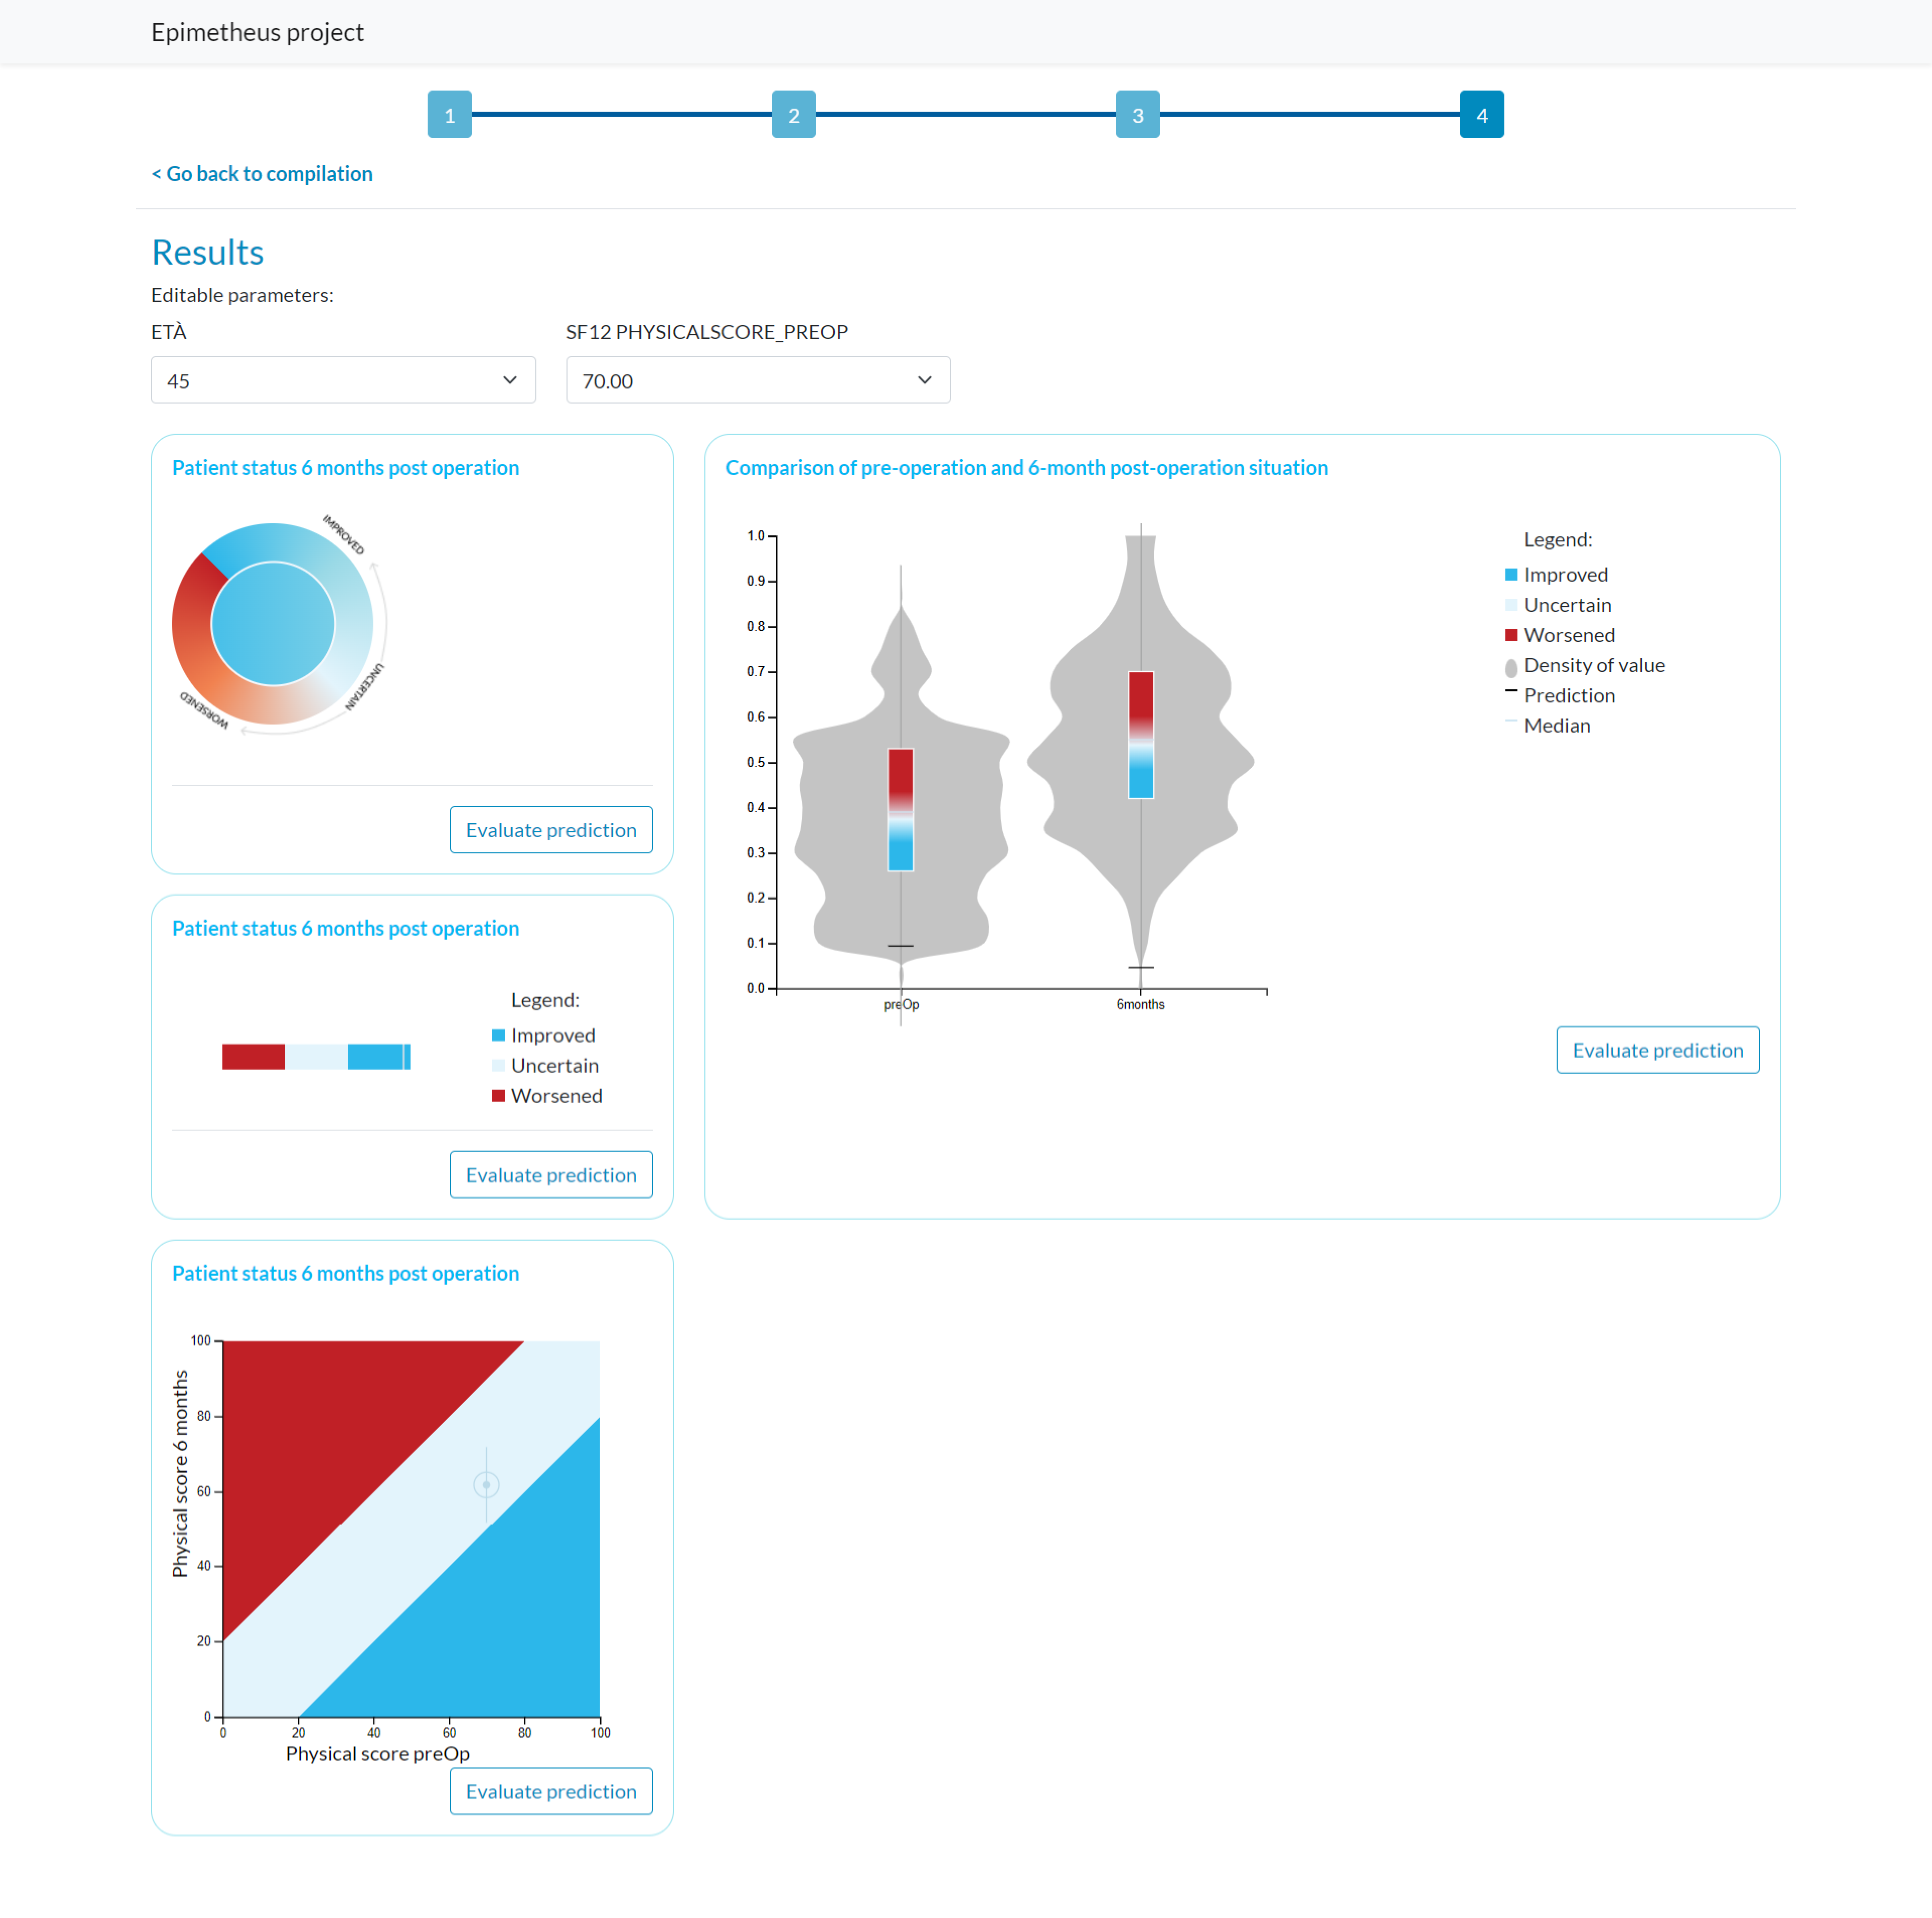
\includegraphics[width=0.7\columnwidth]{epi-start-results} 
%     \caption{Pagina di risultati pre-modifiche}
%     \label{fig:epi-start-results}
% \end{figure}

\begin{figure}[htbp]
    \centering
    \begin{minipage}{0.45\textwidth}
        \centering 
    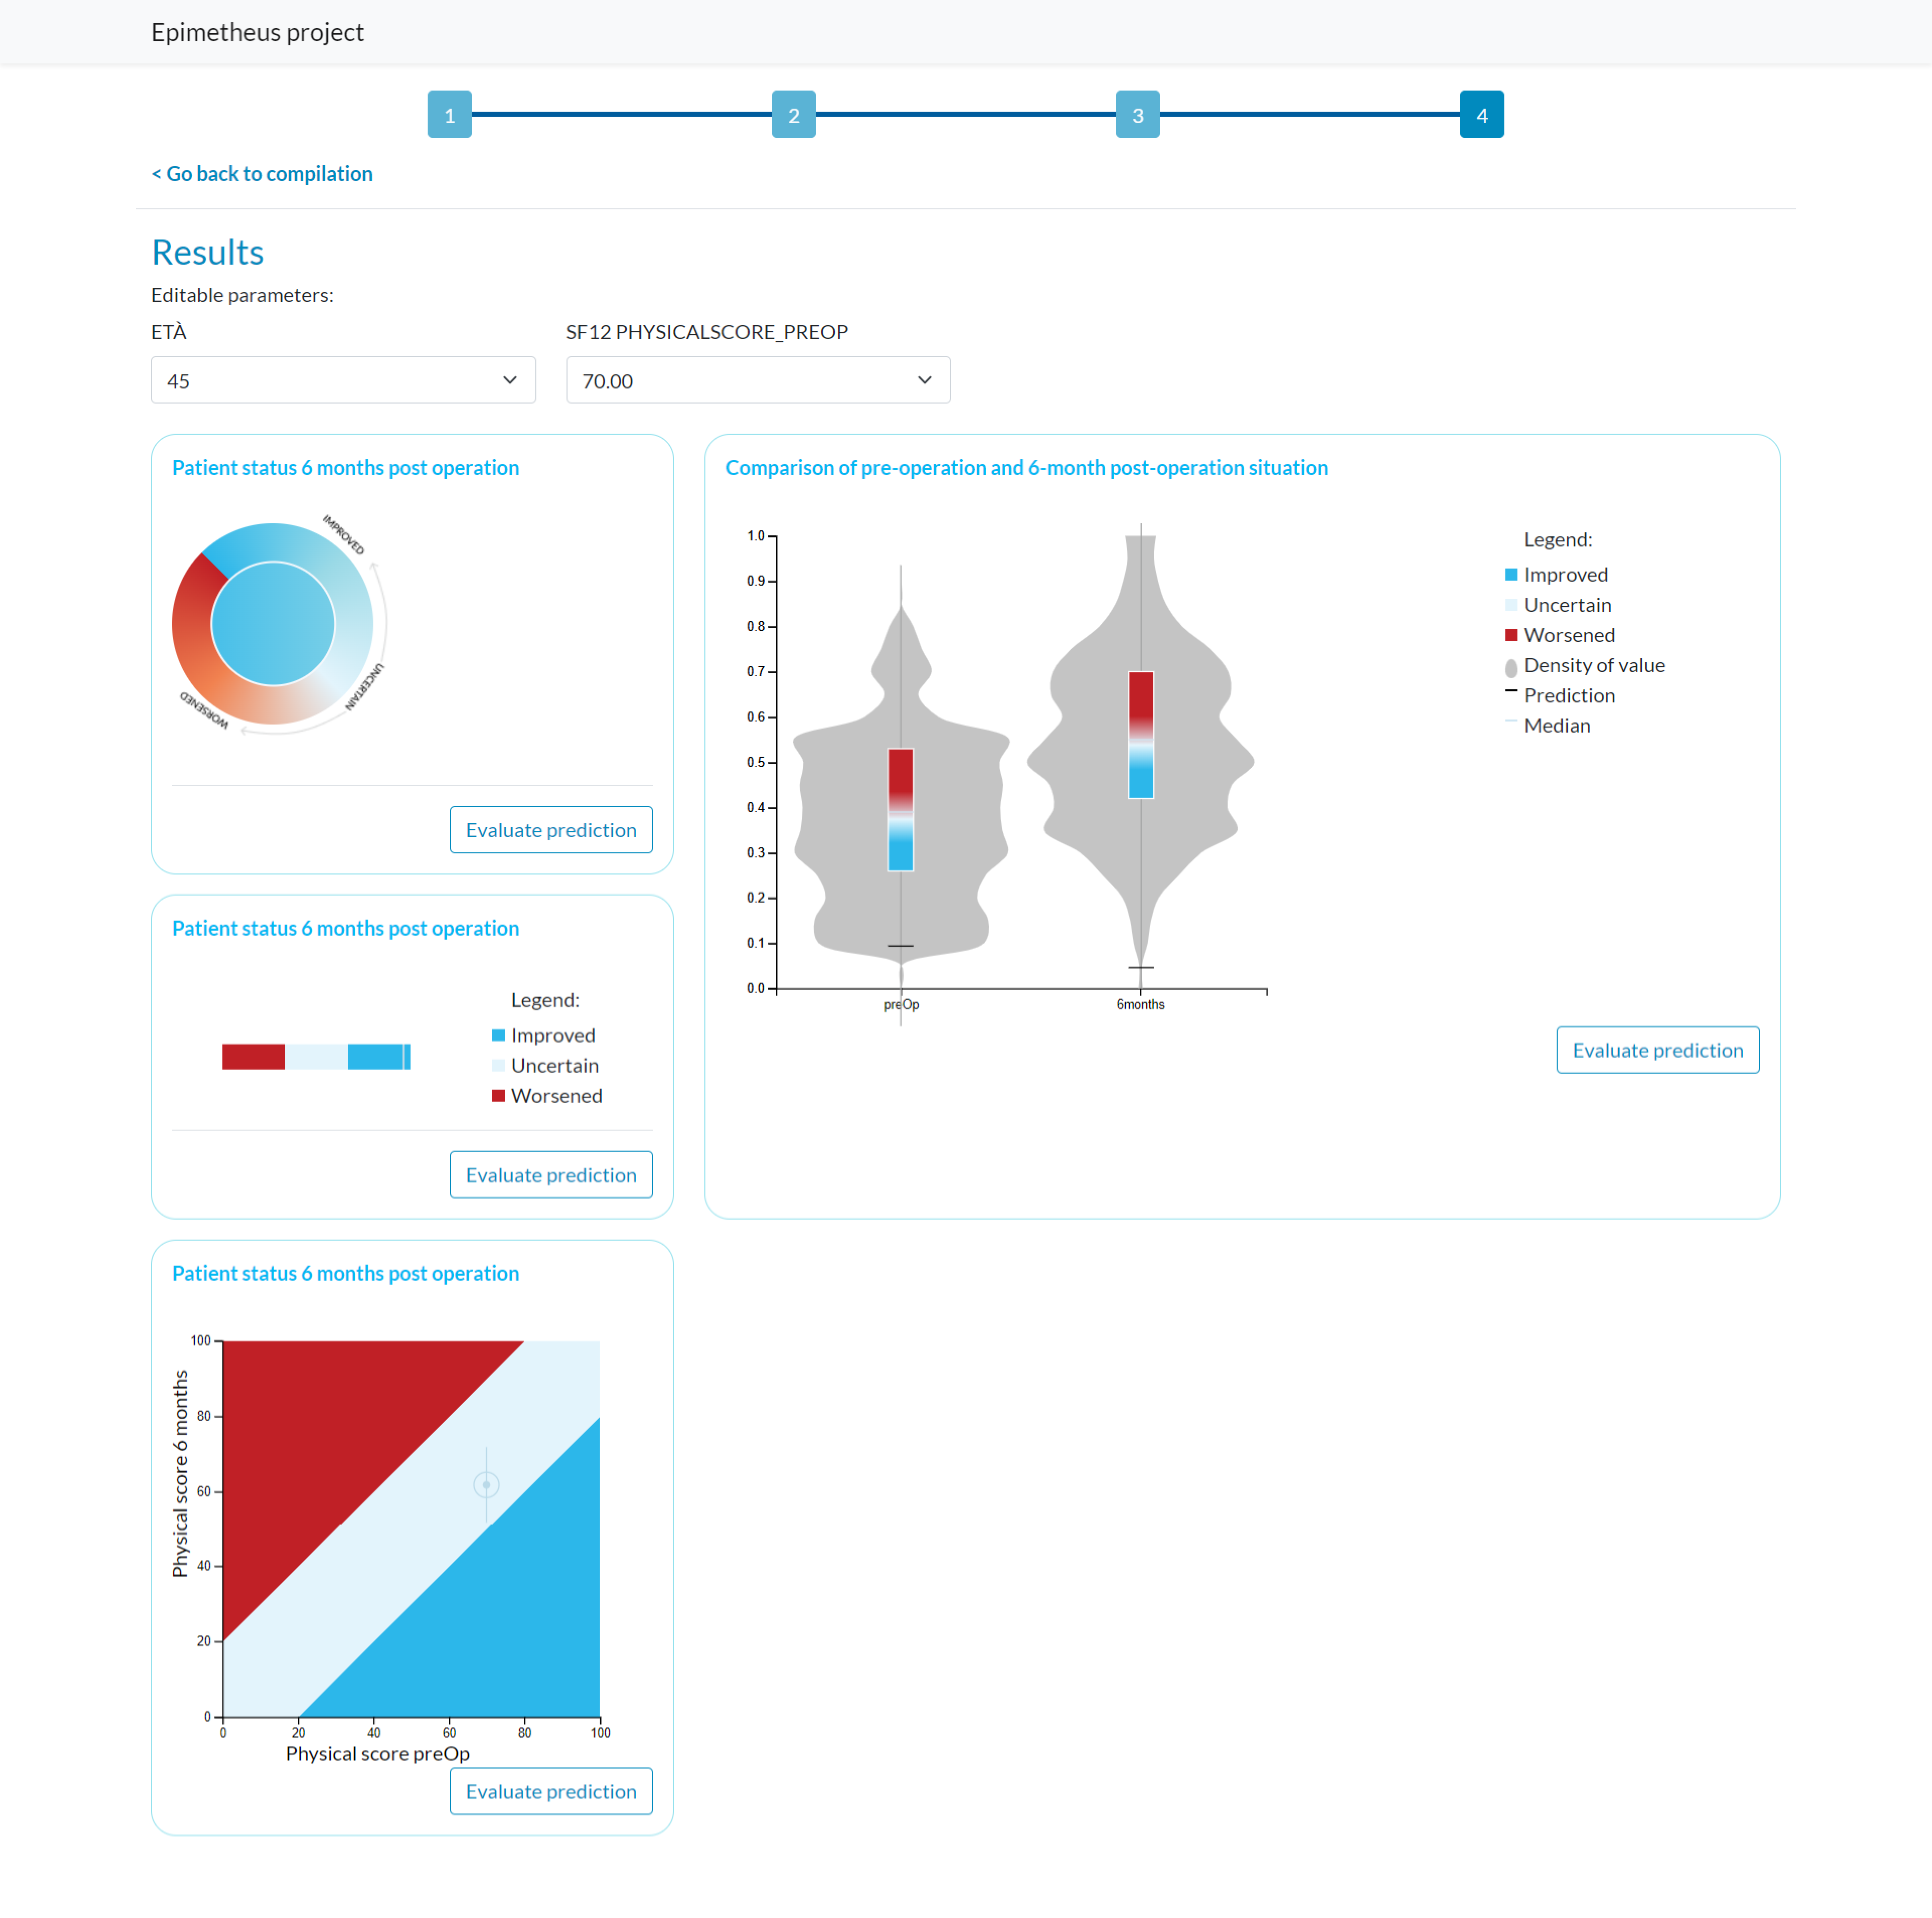
\includegraphics[width=1\columnwidth]{epi-start-results} 
    \caption{Pagina di risultati pre-modifiche}
    \label{fig:epi-start-results}
    \end{minipage}\hfill
    \begin{minipage}{0.45\textwidth}
        \centering 
    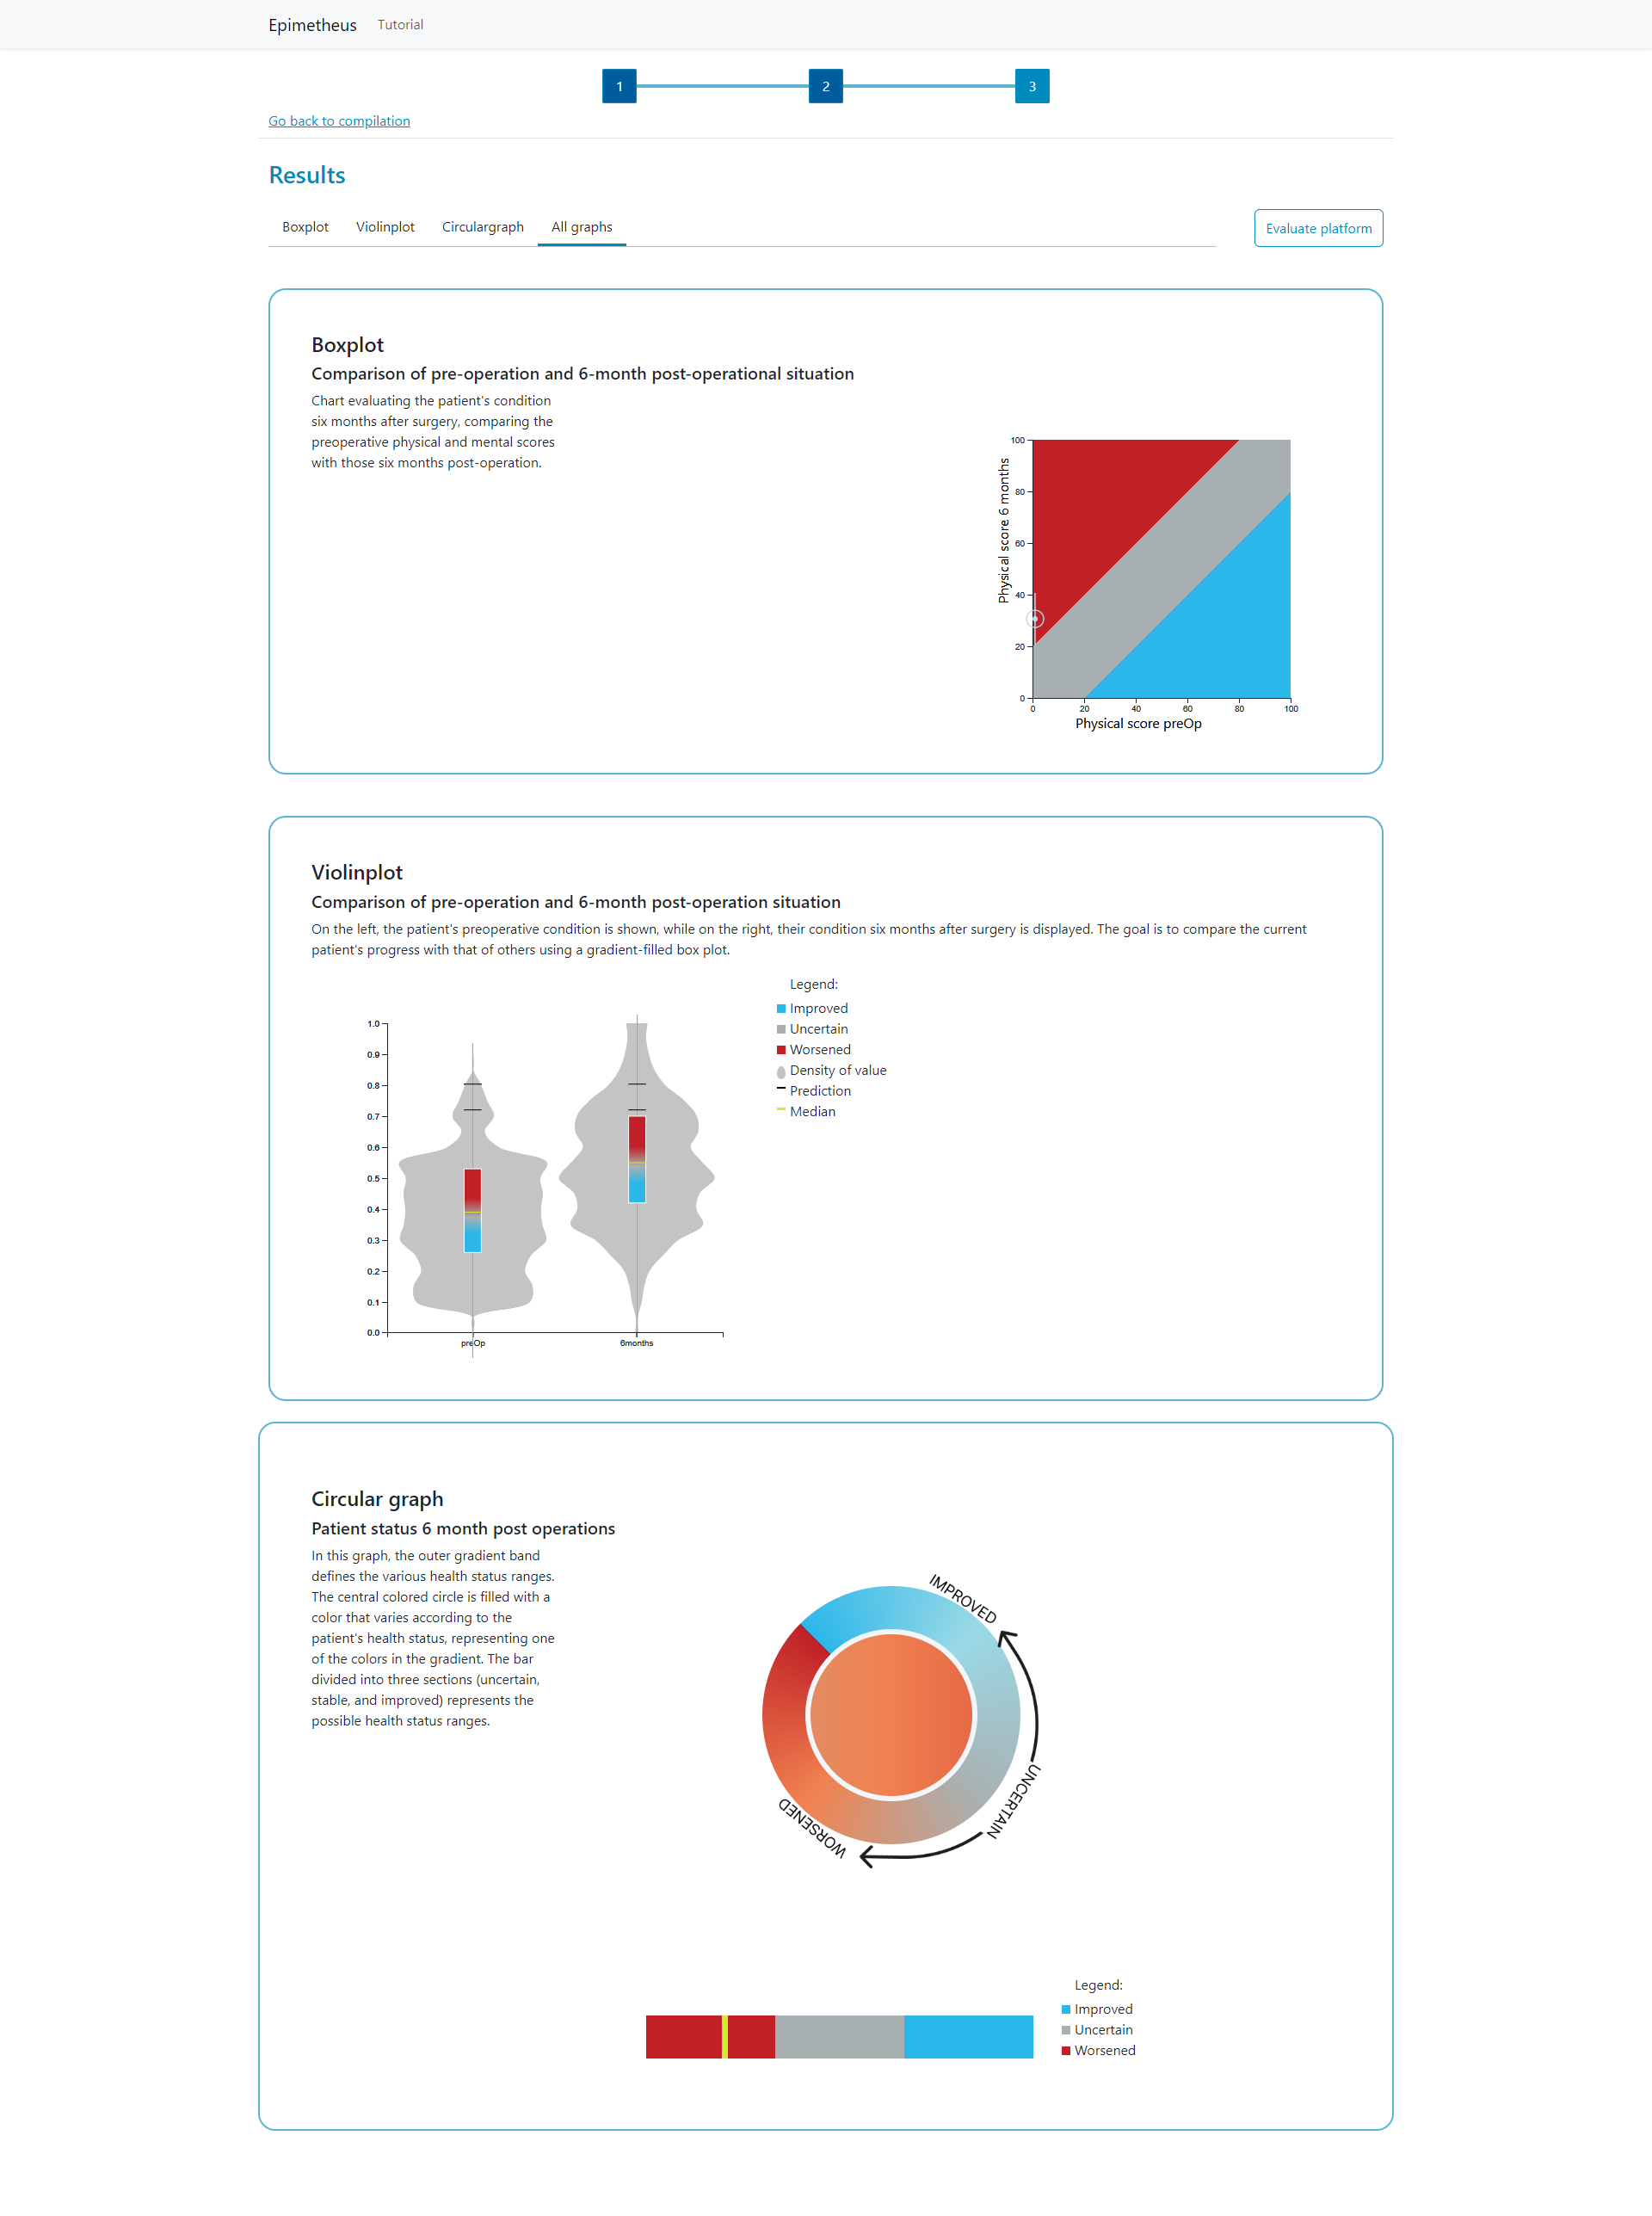
\includegraphics[width=1\columnwidth]{epi-all-graphs} 
    \caption{Pagina di risultati post-modifiche}
    \label{fig:epi-all-graphs}
    \end{minipage}
\end{figure}

\section{Modifiche apportate}

Nella transizione da POC a software completo, il numero di pagine è aumentato: una per il wizard, una per i risultati, una per la valutazione dell'utente circa la piattaforma, e una per il tutorial. Il tutorial è stato posizionato nell'header per garantire un facile accesso da parte dell'utente in qualsiasi momento. Inoltre, il wizard è stato semplificato, eliminando uno step.\\
La pagina dei risultati ha subito le modifiche più significative. È stato inserito un tabbar che permette all'utente di cambiare le visualizzazioni. L'ordine del tabbar è stato progettato in modo tale che l'utente possa vedere prima le singole visualizzazioni e poi tutte insieme in una vista complessiva (\ref{fig:epi-all-graphs}). Quando si clicca sul tab "All graphs", appare un modale bloccante, che l'utente non può chiudere senza prima compilare il form contenuto al suo interno. Questo form deve essere compilato solo una volta ed è cruciale per raccogliere dati sull'utilità percepita dal medico quando visualizza i grafici.\\
È possibile accedere a un altro form tramite il pulsante "Evaluate platform" posizionato in linea con il tabbar. Questo form raccoglie feedback sull'utilità percepita del software nel suo complesso.\\

% \begin{figure}[!ht] 
%     \centering 
%     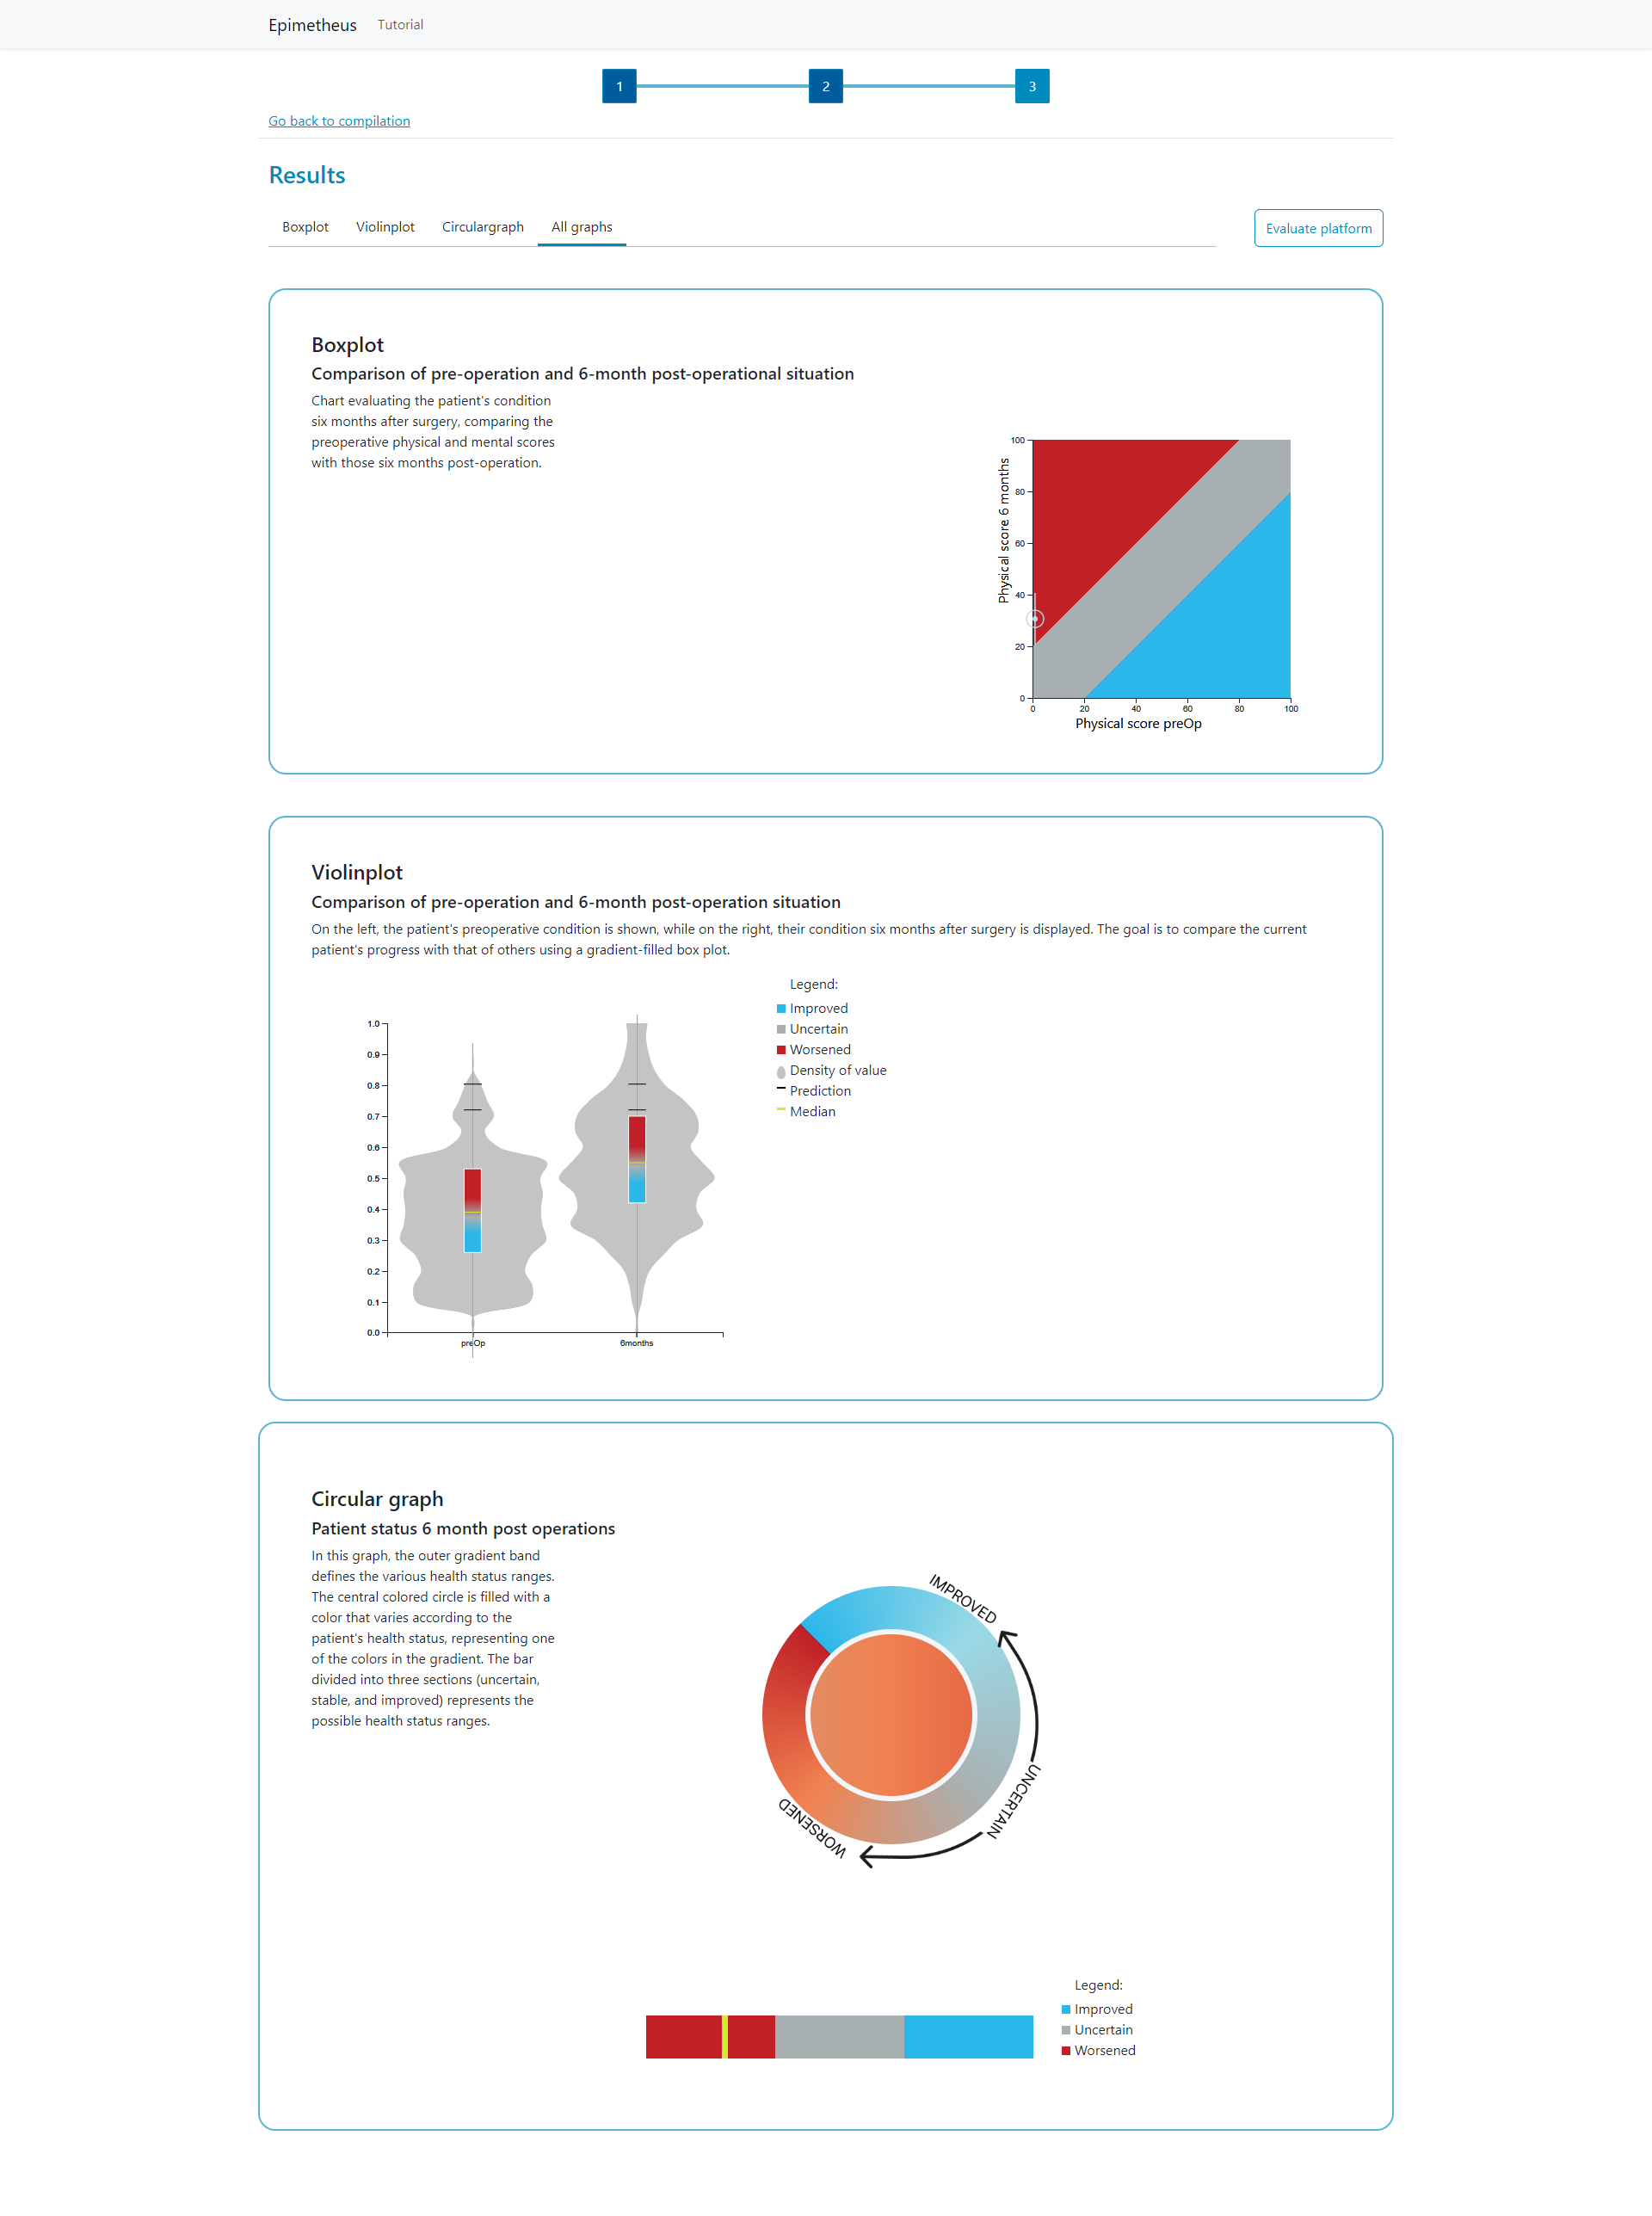
\includegraphics[width=0.7\columnwidth]{epi-all-graphs} 
%     \caption{Pagina di risultati post-modifiche}
%     \label{fig:epi-all-graphs}
% \end{figure}

I grafici sono interattivi, permettendo all'utente di modificare parametri specifici, come il valore del peso, con conseguente ricalcolo del grafico (\ref{fig:editable-parameters}).\\ 

\begin{figure}[!ht] 
    \centering 
    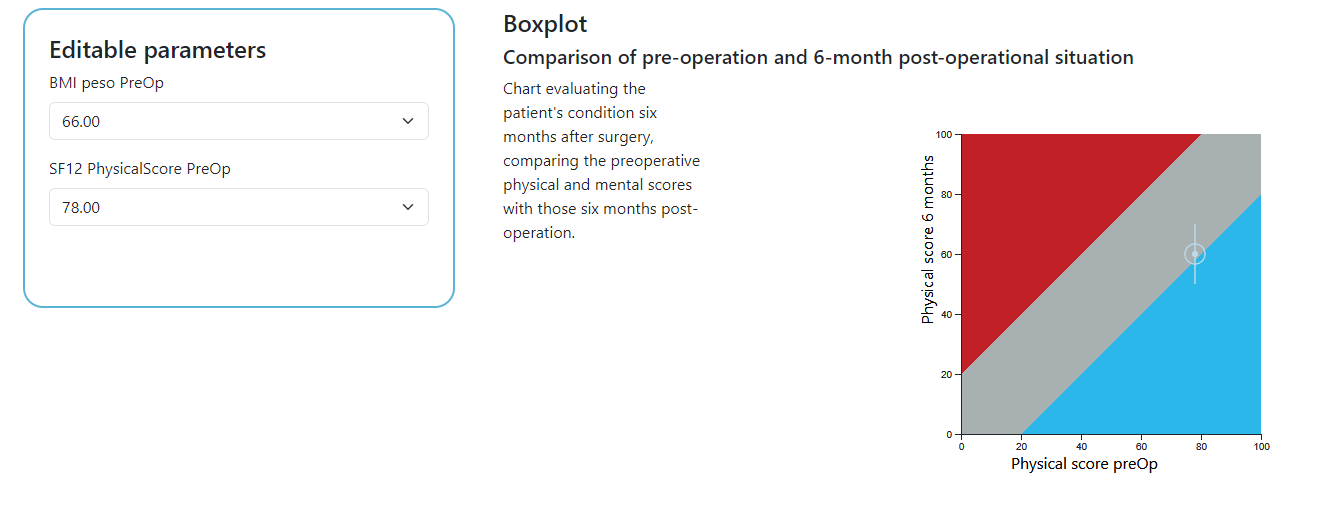
\includegraphics[width=0.9\columnwidth]{editable-parameters} 
    \caption{Esempio di parametri modificabili nel caso del physical score}
    \label{fig:editable-parameters}
\end{figure}

Per quanto riguarda il Visual Design del prodotto ho seguito lo stile iniziale, mantenendo come colore primario il celeste, e uno stile complessivamente fresco e pulito grazie all'adozione del Material Design. Ho usato strategicamente le common region per dividere i vari elementi, soprattutto nella pagina di risultati dove sono visibili tutti i grafici. 
Sono state inoltre apportate modifiche ai colori dei grafici: inizialmente, il colore dell'incertezza era il celeste, ma poiché questo è il colore primario del brand identity del prodotto, ho proposto di sostituirlo con il grigio. Il grigio, per definizione, si presta meglio a rappresentare il dubbio e l'incertezza. A supporto della mia tesi, test condotti su un campione demograficamente variegato hanno confermato che il grigio è percepito come colore "incerto" (\ref{fig:domanda-colore-incertezza}).\\

Non è mancata l'attenzione verso l'accessibilità del prodotto: il nuovo gradiente è stato testato su tutti i livelli di daltonismo rivelando una buona lettura per quasi tutti i livelli di daltonismo (\ref{fig:test-daltonismo}). 

\begin{figure}[!ht] 
    \centering 
    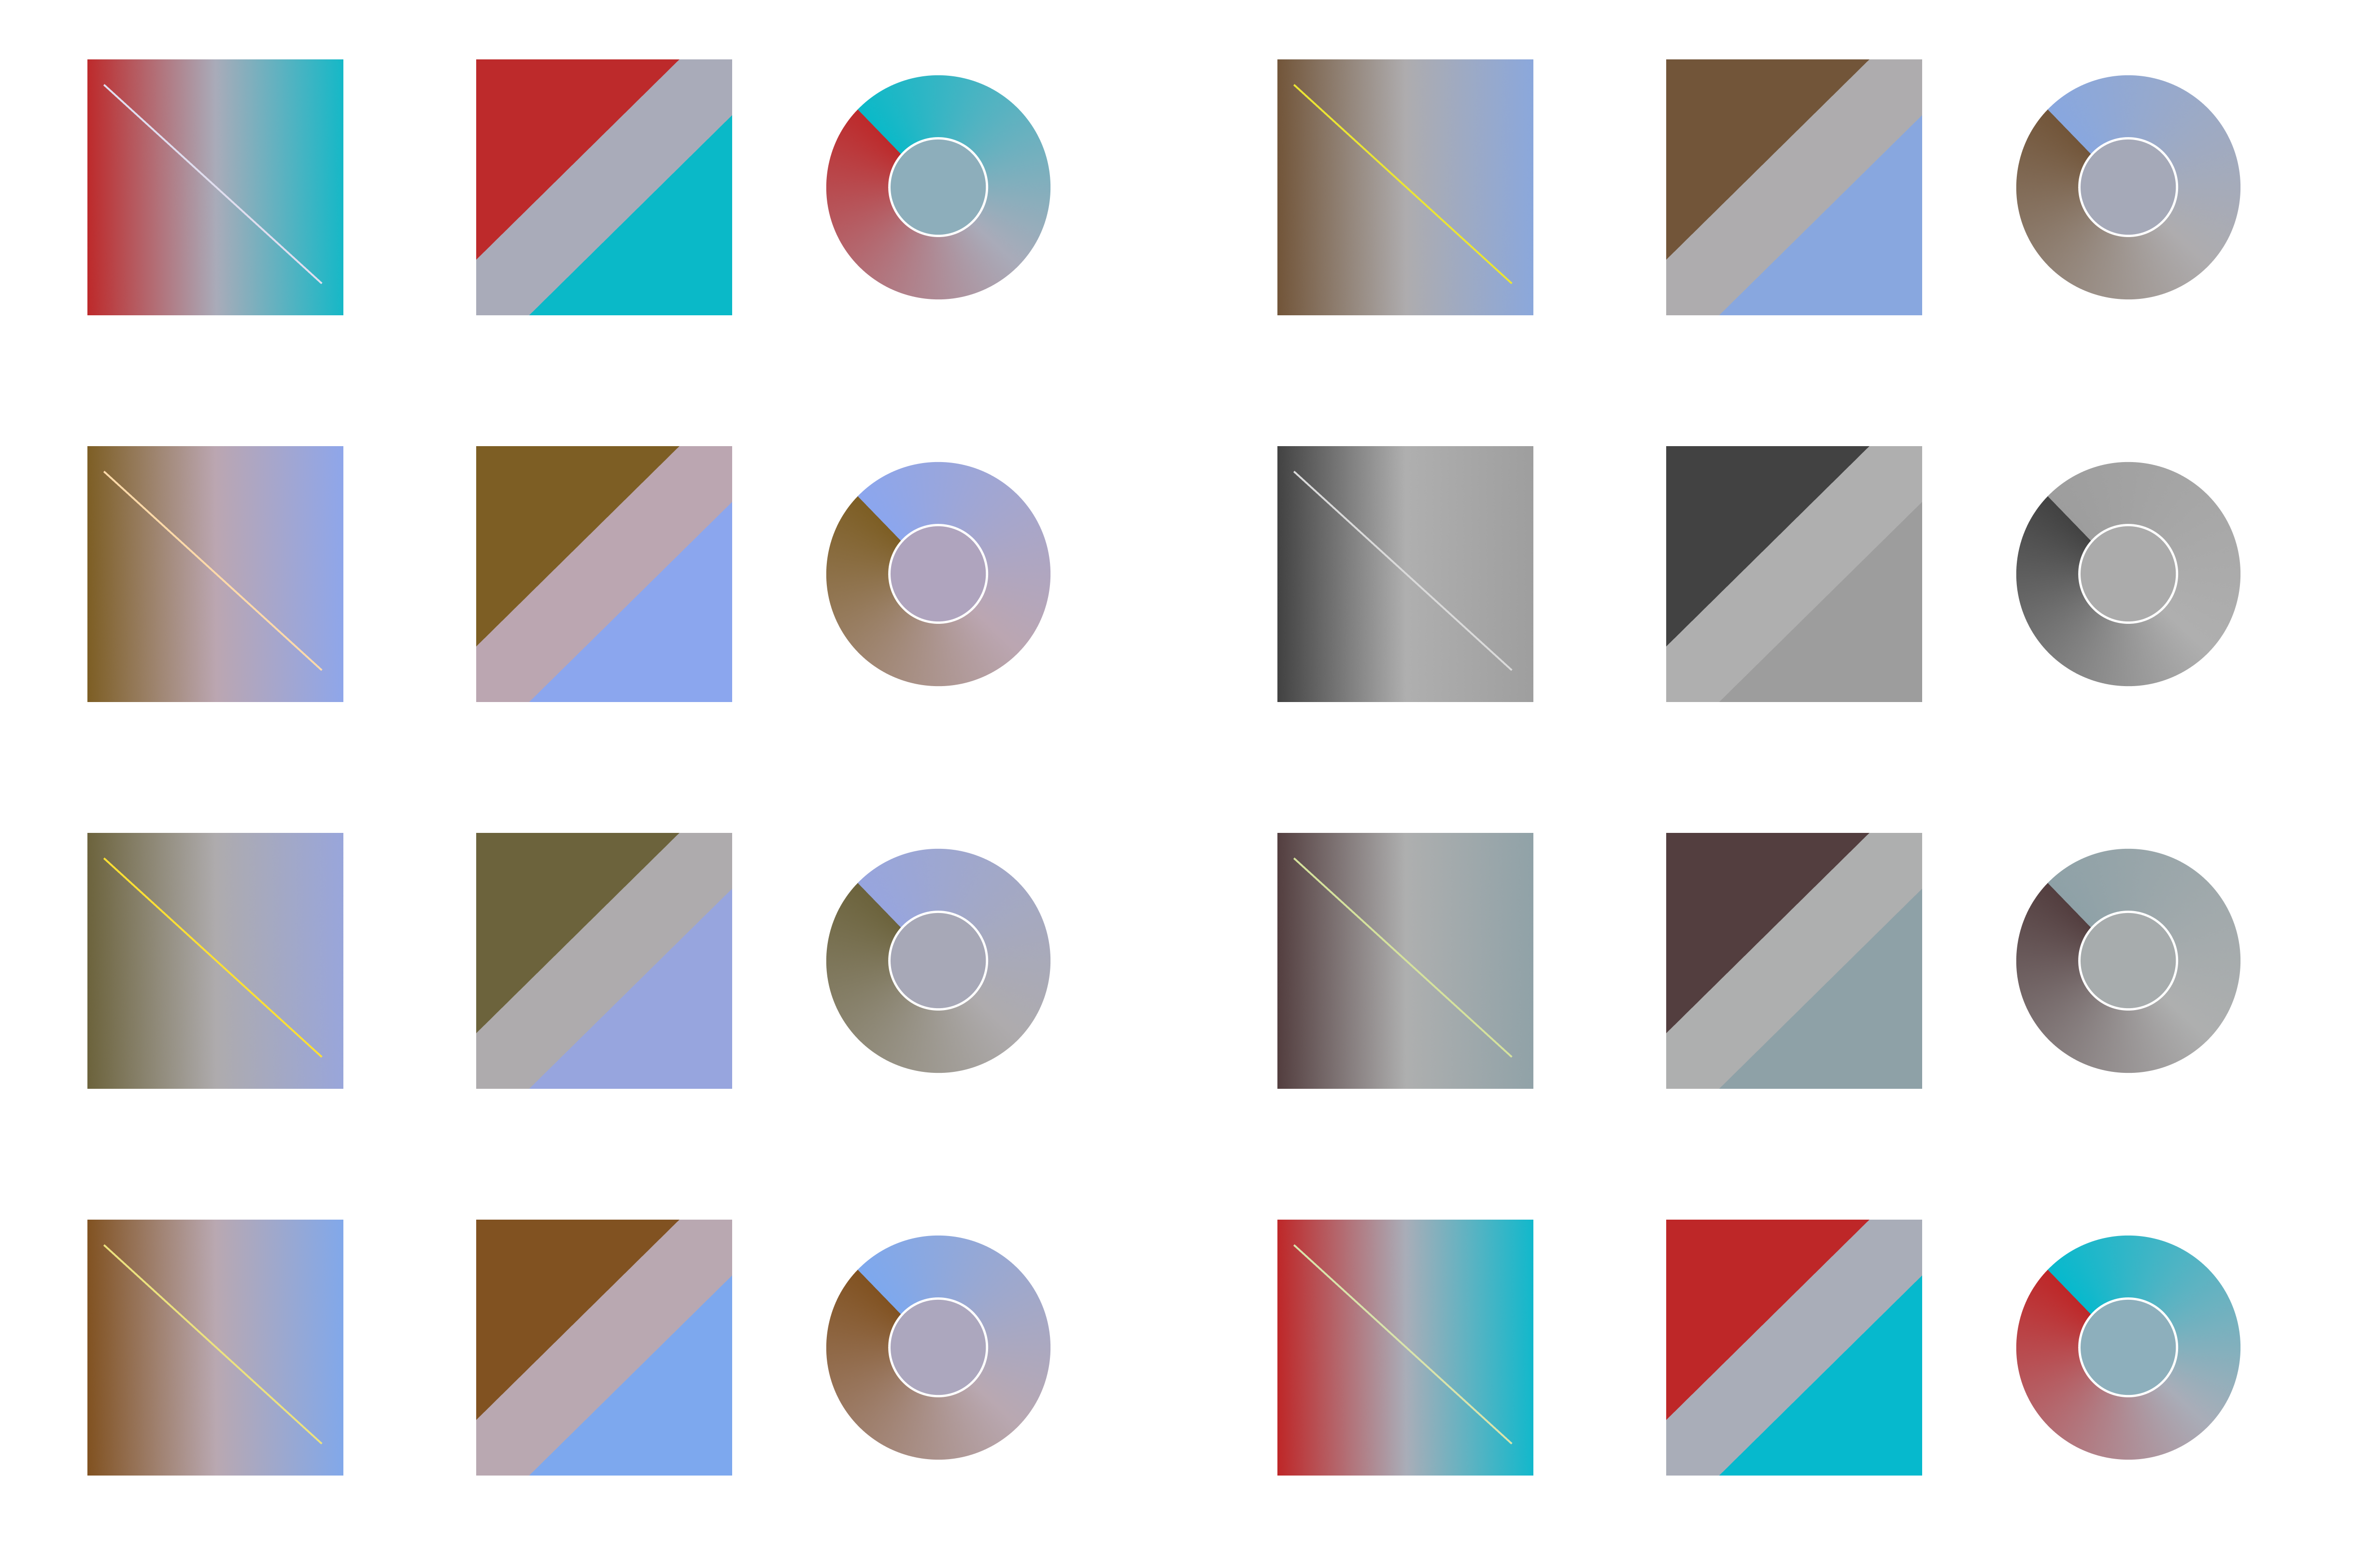
\includegraphics[width=0.5\columnwidth]{test-daltonismo} 
    \caption{Esempio di gradiente e grafico presente in Epimetheus testati con tutti i livelli di daltonismo presenti}
    \label{fig:test-daltonismo}
\end{figure}

\section{Test}
Sono stati condotti due tipi di test, un questionario volto a fornire dati quantitativi e qualitativi, e dei think aloud volti a fornire dati qualitativi. \\

\subsection{Questionario}
\begin{wrapfigure}{r}{0.5\textwidth}
    \centering
    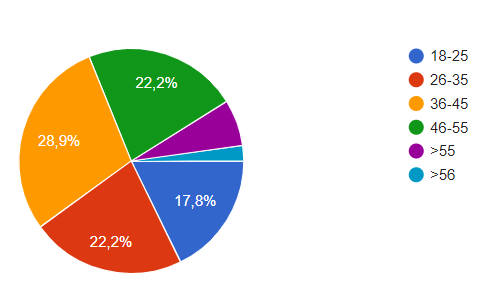
\includegraphics[width=0.6\textwidth]{eta-questionario}
    \caption{Età degli utenti che hanno risposto al questionario}
    \label{fig:eta-questionario}
\end{wrapfigure}

Il questionario è stato somministrato a 45 utenti di diversa età ed estrazione sociale (Figura \ref{fig:eta-questionario}). Tra le prime domande che sono state poste vi è la domanda se sono soliti ad consultare grafici o infografiche nell'ambito del loro lavoro o per interesse personale; circa il 42\% di loro ha risposto di si, il 53\% di loro ha risposto di no. Successivamente si è indagato se gli utenti si ritengono esperti in grafici, il 47\% di loro ha risposto "abbastanza", il 36\% di loro ha risposto "non molto". La maggior parte degli utenti sceglie come fonte da cui visualizzare grafici siti web e libri di testo (Figura \ref{fig:consultazione-grafici}).\\

\begin{figure}[!ht] 
    \centering 
    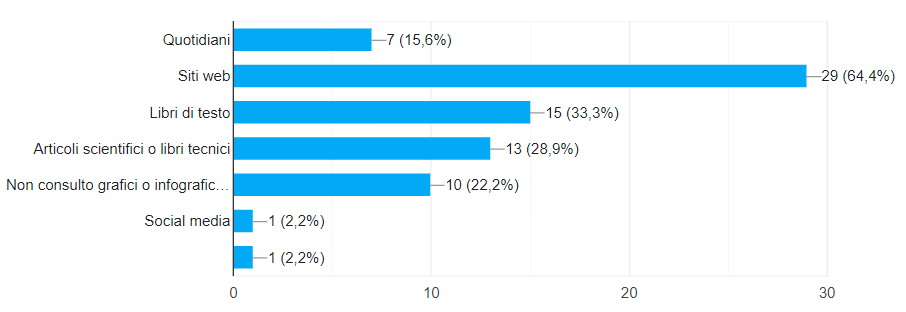
\includegraphics[width=1\columnwidth]{consultazione-grafici} 
    \caption{Principali fonti da cui gli utenti consultano grafici o infografiche}
    \label{fig:consultazione-grafici}
\end{figure}

Successivamente il questionario si è articolato su domande relative ai colori e ai grafici. Qui si è indagato su come gli utenti percepiscono l'incertezza, quindi è stat posta una prima domanda volta a capire se la scelta del grigio invece dell'azzurro comunicasse meglio il concetto di incertezza (Figura \ref{fig:gradienti-a-confronto}). 

\begin{figure}[!ht] 
    \centering 
    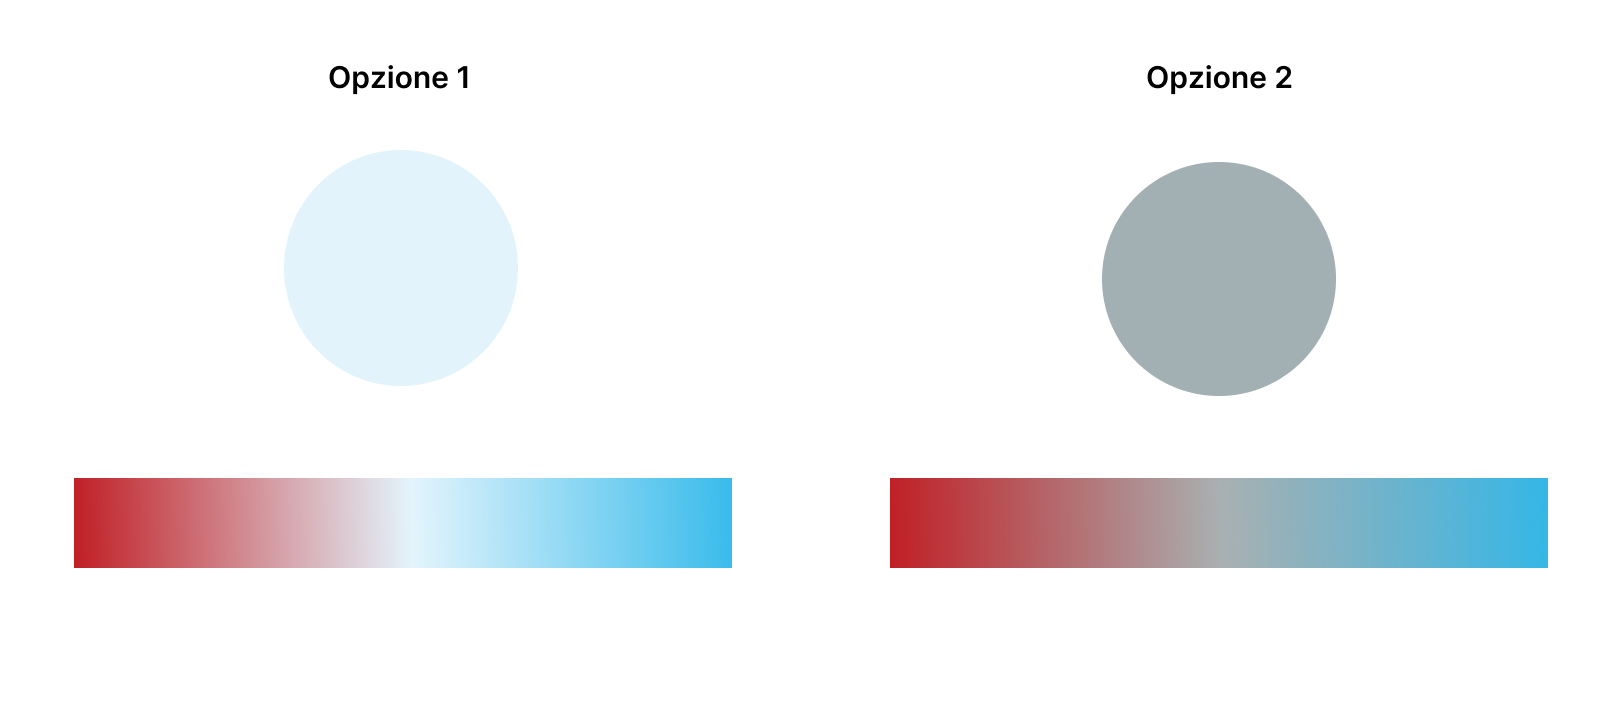
\includegraphics[width=0.6\columnwidth]{gradienti-a-confronto} 
    \caption{I due gradienti messi a confronto, con focus posto sull'area centrale che rappresenta l'incertezza. Il primo gradiente è quello inzialmente presente sul progetto, il secondo è quello che si vuole adottare}
    \label{fig:gradienti-a-confronto}
\end{figure}


\begin{figure}[!ht] 
    \centering 
    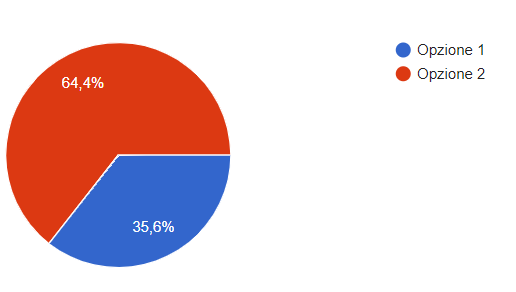
\includegraphics[width=0.4\textwidth]{domanda-colore-incertezza}
    \caption{Distribuzione delle risposte alla domanda che mette a confronto i due gradienti}
    \label{fig:domanda-colore-incertezza}
\end{figure}

Ne è emerso che l'intuizione era corretta, infatti il 64\% ha affermato di percepire maggiore incertezza utilizzando il colore grigio invece che azzurro (Figura \ref{fig:domanda-colore-incertezza}). \\

In un'altra sezione si è indagato sulla percezione dell'incertezza nell'ambito del grafico "Circulargraph". In particolare si voleva capire se effettivamente gli utenti percepissero correttamente lo stato di salute che si voleva comunicare (Figura \ref{fig:domande-circulargraph}). Per condurre questo test sono state realizzate alcune copie del grafico, il colore del cerchio centrale è stato prelevato a partire da vari punti del gradiente esterno. Successivamente all'interno del questionario sono stati disposti i grafici in maniera casuale, in modo tale che l'utente non avesse un bias di ordine. \\

\begin{figure}[!ht] 
    \centering 
    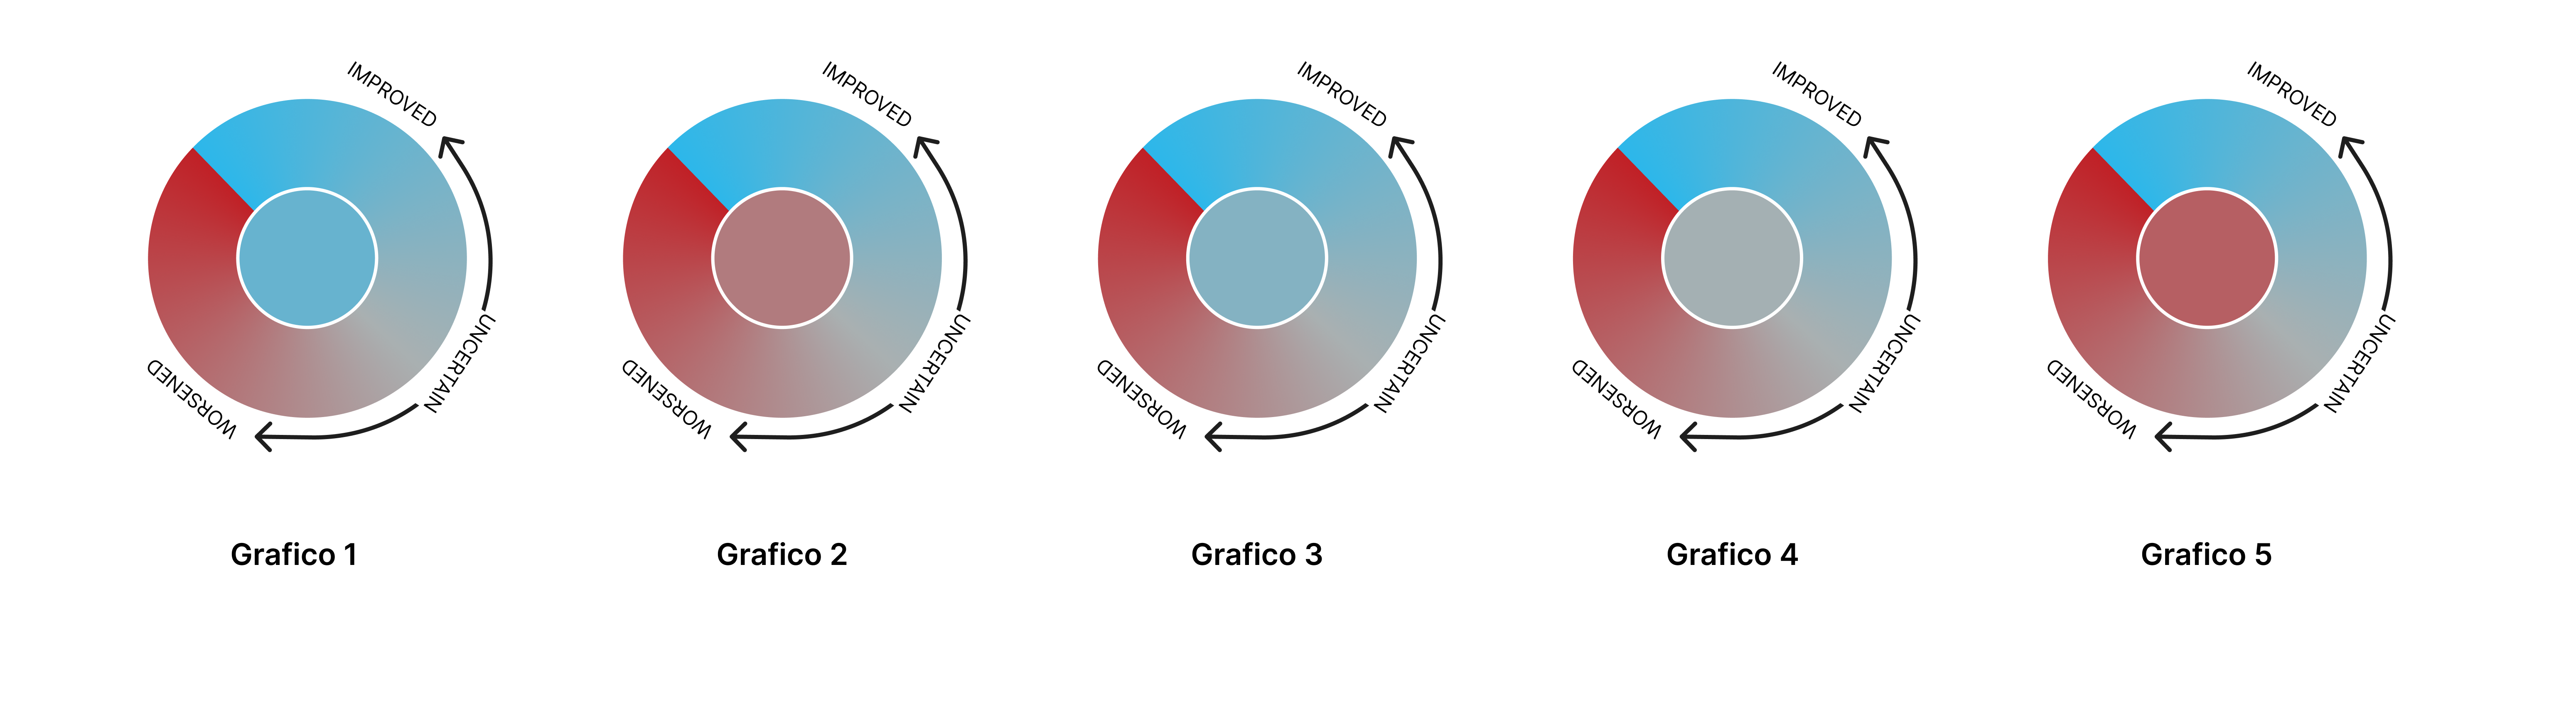
\includegraphics[width=0.9\textwidth]{domande-circulargraph}
    \caption{I circulargraph sottoposti a quesito}
    \label{fig:domande-circulargraph}
\end{figure}

I risultati sono stati i seguenti:
\begin{itemize}
    \item Nel grafico 1 il 44\% degli intervistati ritiene che il paziente avrà un discreto miglioramento; il 44\% ritiene che avrà un netto miglioramento;
    \item Nel grafico 2 il 77\% degli intervistati ritiene che il paziente avrà un discreto peggioramento;
    \item Nel grafico 3 il 66\% degli intervistati ritiene che il paziente avrà un discreto miglioramento, il 22\% ritiene che avrà un esito incerto;
    \item Nel grafico 4 l'84\% degli intervistati ritiene che il paziente avrà un esito incerto, non si può dire se migliorerà o peggiorerà;
    \item Nel grafico 5 il 49\% degli intervistati ritiene che il paziente avrà un netto peggioramento, mentre il 38\% ritiene che avrà un discreto peggioramento.
\end{itemize}
Le conclusioni che si possono trarre da questi dati sono che il colore centrale effettivamente comunica correttamente quale sarà lo stato di salute del paziente. Inserire una legenda che permetta di capire quale è il colore del miglioramento e quale è il colore del peggioramento fornisce ulteriori indicazioni all'utente per orientarsi. \\

Ultima domanda ha riguardato un test A/B, in particolare si è messo a paragone le due pagine di risultati pre (opzione 1) e post (opzione 2) modifiche, e si è chiesto agli utenti quali delle due opzioni preferissero e perchè. Il 93\% dei partecipanti ha affermato di preferire la nuova interfaccia di risultati (Figura \ref{fig:risposte-test-ab}); i motivi riportati sono stati vari, tra i principali si può citare come motivazione una maggiore pulizia dell'interfaccia, l'interfaccia è meno stancante alla vista, è più ordinata, il commento che accompagna i grafici ne favorisce la comprensione. La parola più frequente è stata "lineare". \\

\begin{figure}[!ht] 
    \centering 
    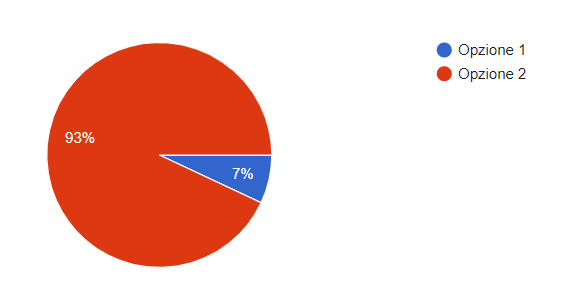
\includegraphics[width=0.5\textwidth]{risposte-test-ab}
    \caption{Risposte al test A/B che paragona l'interfaccia iniziale con la finale}
    \label{fig:risposte-test-ab}
\end{figure}

Tra questi vi è un commento in particolare che vale la pena citare: 
\begin{quote}
    \textit{Se l'intento è quello di avere un quadro chiaro e completo del paziente la prima opzione è la migliore perché sono visualizzate più informazioni in poco spazio, dando un quadro generale dello stato di salute; si perde però il dettaglio o delle note che potrebbero risultare comunque interessanti in caso di pazienti/operazioni particolari che invece nella seconda opzione potrebbero essere più facili da individuare.}
\end{quote}
Questo commento lascia intendere che in futuro si potrebbe aggiungere un bottone che modifichi il layout dell'interfaccia, in modo tale da avere una visualizzazione raggruppata oppure una visualizzazione a lista.

\subsection{Think aloud}
Sono stati condotti dei test di usabilità con utenti appartenenti all'ambito medico.
I task richiesti agli intervistati sono stati:
\begin{itemize}
    \item compilare il form contenente i dati e accedere alla pagina di risultati
    \item modificare le dimensioni su cui indagare
    \item accedere alla pagina divalutazione piattaforma
    \item tornare alla pagina del wizard e compilare un nuovo questionario 
\end{itemize}

Per tutti i partecipanti sono stati condotti due test, uno con score physical (che chiameremo test Alfa) e uno con score mental (che chiameremo test Beta).
I dati utilizzati per i partecipanti sono stati gli stessi, in particolare il test Alfa indagava lo stato di salute di un paziente con un physical score pre operation alto e un mental score pre operation discreto, il test Beta indagava lo stato di salute di un paziente con physical score e mental score pre operation molto bassi. Entrambi davano esiti incerti più o meno definiti, quindi si è chiesto ai partecipanti se avrebbero operato o no il paziente. È stata lasciata libera scelta sul tipo di operazione da esplorare. 

\subsubsection{Partecipante A}
Il partecipante A è un medico ortopedico specializzato nelle protesi all'anca e al ginocchio.
Durante l'utilizzo del software l'utente si è mosso agilmente all'interno delle pagine. Le funzionalità sono apparse chiare e intuitive, non ha riscontrato difficoltà di sorta nel portare a termine i suoi task. \\
Dopo un contesto iniziale sulla prima visualizzazione, ha ritenuto il grafico chiaro, è stato in grado di interagire con i parametri modificabili per verificare come lo stato di salute del paziente potesse cambiare nel post operatorio. La seconda visualizzazione (il violinplot) è stata ritenuta molto buona. È stata valutata come comprensibile, chiara, dava precise indicazioni sullo stato di salute del paziente nel post operatorio. La terza visualizzazione (il circulargraph e il boxplot) è stata valutata abbastanza positivamente. Il boxplot è stato ritenuto molto chiaro ed esplicito, il circulargraph invece è stato ritenuto meno ovvio da comprendere. \\ 

\begin{figure}[htbp]
    \centering
    \begin{minipage}{0.45\textwidth}
        \centering
        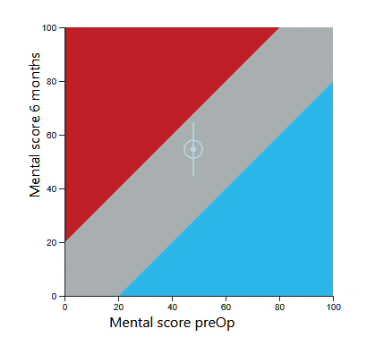
\includegraphics[width=0.8\textwidth]{partecipante-a-test-beta-boxplot}
        \caption{Boxplot del test Beta condotto dal partecipante A}
        \label{fig:boxplot-partecipante-a}
    \end{minipage}\hfill
    \begin{minipage}{0.45\textwidth}
        \centering
        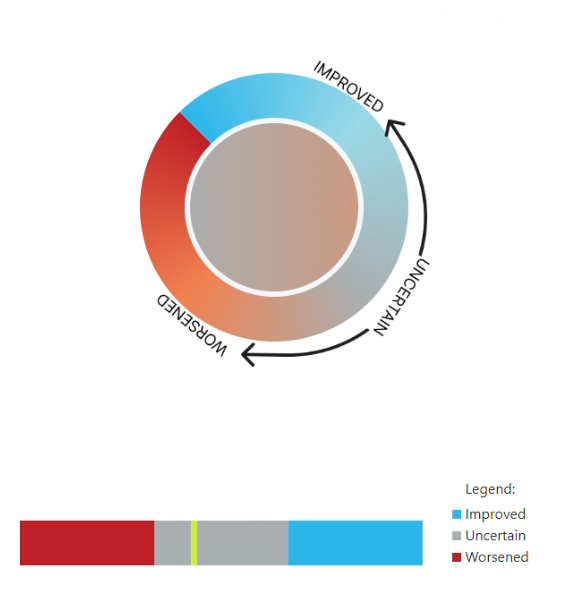
\includegraphics[width=0.8\textwidth]{partecipante-a-test-beta-circulargraph}
        \caption{Circulargraph del test Beta condotto dal partecipante A}
        \label{fig:circulargraph-partecipante-a}
    \end{minipage}
    \caption*{In questo test si è indagato l'ambito dell'operazione all'anca}
\end{figure}

L'opinione generale nei confronti dell'interfaccia è stata molto positiva, l'utente l'ha definita facilissima da comprendere. Tuttavia, quando si è chiesto di tornare alla pagina iniziale per tentare una nuova indagine, l'utente ha riscontrato difficoltà nell'individuare il link che portasse alla prima pagina. \\
Al secondo questionario (test alfa) compilato si è andato ad indagare l'opinione del medico nei confronti dei grafici. Nonostante i grafici dessero un esito incerto ((Figura \ref{fig:boxplot-partecipante-a}), (Figura \ref{fig:circulargraph-partecipante-a})) il medico ha affermato che opererebbe il paziente in quanto terrebbe conto dello stato mentale del paziente in relazione al suo dolore fisico. Quindi di fatto la sua opinione non è stata influenzata dal grafico. Secondo il partecipante, infatti, un paziente può avere un mental score negativo perchè sta male, ma se a seguito di un'operazione il suo dolore scomparisse allora il suo mental score migliorerebbe. Il partecipante ha riferito che se il fattore predittivo tenesse conto dell'interazione tra la VAS e lo stato mentale del paziente il grafico sarebbe molto più affidabile.\\
L'utente ha sollevato inoltre che sarebbe opportuno mettere dei target del dolore percepito nel post operatorio, così da sfruttarli nell'ambito delle predizioni. Ha fatto notare inoltre che nell'ambito dello stato mentale del paziente è importante indagare anche su due fattori: il primo è il tempo intercorso tra la prima comparsa del dolore fisico ad oggi, la seconda di come si sente a seguito della lista d'attesa per l'operazione. Infatti pazienti che stanno male e che sono posti di fronte ad una lista d'attesa lunga hanno un peggioramento del loro mental score. \\
Una lode fatta dal medico riguarda il fatto che tra i parametri modificabili dei grafici figurano parametri concreti su cui effettivamente si può intervenire. Una mia domanda è stata se ritiene che le dimensioni disponibili su cui indagare siano appropriate a formare un'opinione circa lo stato di salute a 6 mesi dall'operazione. La risposta è stata si, e che varrebbe la pena aggiungere l'HOOS (Hip disability and Osteoarthritis Outcome Score), il KOOS (Knee Disability and Osteoarthritis Outcome Score), e il VAS. Attualmente HOOS e KOOS non esistono nel calcolo predittivo operato dal backend, quindi questo suggerimento si configura come uno sviluppo futuro. \\
Un'altra domanda che è stata fatta riguarda la modalità di inserimento dei dati: è stato chiesto se l'utente ritiene più facile avere questi valori numerici da copiare nell'apposito input text, oppure se sia meglio presentare il PROM vero e proprio e lasciare che l'utente lo compili così come è stato compilato dal paziente. L'utente ha risposto che l'attuale modalità di inserimento dei dati è preferibile. Sarebbe ancora più preferibile avere accesso al registro dei dati che ha a disposizione l'istituto Galeazzi. 


\subsubsection{Partecipante B}
\label{partecipante-b}
Il partecipante B è un tecnico audioprotesista; sebbene non sia un medico ortopedico, questo utente si è reso interessante perchè nel suo lavoro affronta tematiche molto simili agli utenti target di Epimetheus, adottando anche metodologie di lavoro simili.\\
Dopo aver spiegato il contesto di utilizzo del software, a partire dall'inserimento dei dati il partecipante è riuscito a portare a termine il wizard senza difficoltà, approdando nella pagina dei risultati. Qui ha interagito con i vari grafici osservandone i cambiamenti ove presenti. Il partecipante ha trovato molto utile la spiegazione contestuale a ciascun grafico, in quanto, soprattutto al primo utilizzo, l'utente inesperto necessita di essere inserito nel contesto applicativo. Ha commentato che i dati sono chiari, le previsioni a 6 mesi dall'operazione si rendono utili a capire come effettivamente cambierà lo stato di salute del paziente anche in relazione al cambiamento dei parametri modificabili. \\

\begin{wrapfigure}{r}{0.4\textwidth}
    \centering
    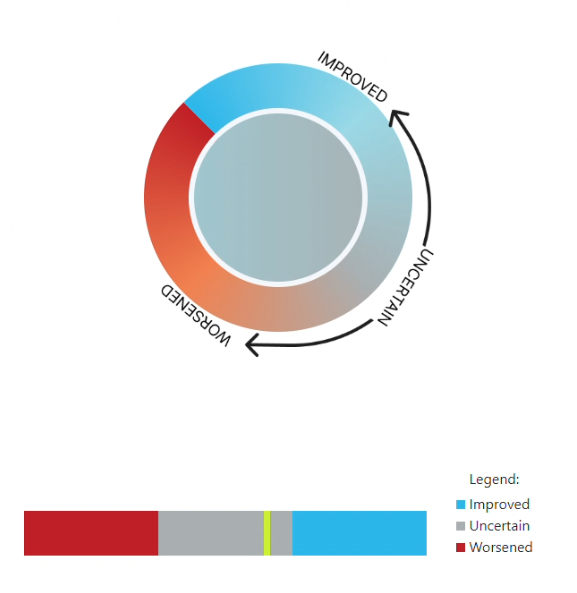
\includegraphics[width=0.4\textwidth]{partecipante-b-test-alfa-circulargraph}
    \caption{Circulargraph del test Alfa condotto dal partecipante B}
    \caption*{In questo test si è indagato l'ambito dell'operazione all'anca}
    \label{fig:circulargraph-partecipante-b}
\end{wrapfigure}

Quando è stato chiesto di tornare alla pagina inziale per condurre un altro test, l'utente ha individuato subito il link per tornare al wizard. Nell'eseguire il nuovo test si è notato come il partecipante aveva già assunto confidenza col prodotto, andando spontaneamente a modificare i parametri necessari per indagare come potesse cambiare lo stato di salute del paziente. Nel secondo test ho chiesto al partecipante se opererebbe il paziente. La risposta è stata di si, perchè se vi è una variazione del peso del paziente il grafico si sposta verso un miglioramento (Figura \ref{fig:circulargraph-partecipante-b}). \\
Il partecipante ha commentato che l'interfaccia è molto rapida da utilizzare e comprendere, non ci sono fronzoli, le informazioni sono tutte disponibili. \\

Dopo il test sul prodotto, il partecipante ha spiegato vari aspetti del suo lavoro. Come tecnico audioprotesista il suo lavoro prevede l'utilizzo di questionari, chiamati COSI (Client Oriented Scale of Improvement), attraverso i quali si va ad indagare quanto il paziente sente, qual è la sua percezione del rumore, se è in grado di distinguere determinati suoni in determinate situazioni, quanto ha disagio in situazioni rumorose (come in mezzo alla folla). Questo test viene effettuato due volte, una volta nel preprotesizzazione, una seconda nel postprotesizzazione, e viene associato a dei test strumentali che forniscono dati numerici. In questa intervista il partecipante ha spiegato che trova difficoltà a comunicare al paziente informazioni concrete e comprensibili circa il suo stato di salute, perchè gli strumenti a disposizione sono pochi e forniscono per lo più dati numerici. Il partecipante ha trovato particolarmente comprensibile Epimetheus, poichè ha ritenuto che il colore fosse molto più comunicativo rispetto ai numeri. Ha inoltre sottolineato che sarebbe estramamente utile nel suo lavoro avere dei grafici che possano confrontare il pre e post protesizzazione, in quanto avrebbe modo di capire e spiegare al paziente quale sarebbe il margine di miglioramento.\\ Infine ha affermato che utilizzerebbe il prodotto con il paziente. 

\subsubsection{Partecipante C}
Il partecipante C è uno studente di medicina e chirurgia. \\
Dopo la spiegazione del contesto iniziale il partecipante si è approcciato con il prodotto in modo naturale.\\
La prima visualizzazione è stata ritenuta chiara a seguito di spiegazioni circa il suo significato, la descrizione circostante ha aiutato la comprensione. La seconda descrizione è apparsa più comprensibile soprattutto a seguito di interazioni con i parametri modificabili. La terza visualizzazione è stata quella più chiara ed esplicita ed è stata quella che ha permesso più facilmente di prendere decisioni in merito allo stato di salute del paziente (Figura \ref{fig:circulargraph-partecipante-c}). \\

\begin{wrapfigure}{r}{0.4\textwidth}
    \centering
    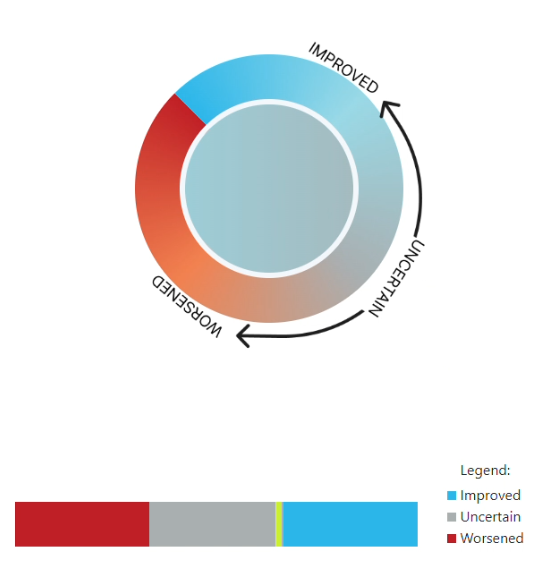
\includegraphics[width=0.4\textwidth]{partecipante-c-test-alfa-circulargraph}
    \caption{Circulargraph del test Alfa condotto dal partecipante C}
    \caption*{In questo test si è indagato l'ambito dell'operazione al ginocchio}
    \label{fig:circulargraph-partecipante-c}
\end{wrapfigure}

In questo contesto si è chiesto al partecipante se opererebbe il paziente e la risposta è stata che dipende. Secondo l'utente, dal momento che il paziente presenta un mental score basso sarebbe opportuno prima chiedere supporto psicologico per aiutare il paziente a migliorare il proprio stato mentale, e successivamente si potrebbe valutare una operazione al ginocchio. Il partecipante C ritiene molto importante avvalersi del supporto di una equipe medica che possa supportare e accompagnare il paziente nel suo percorso di cura. Di fronte l'indecisione la prima scelta sarebbe chiedere un confronto con colleghi. \\
Alla domanda se userebbe il software con il paziente ha risposto di si. \\
Quando è stato chiesto di tornare alla pagina iniziale per condurre una nuova analisi l'utente è stato in grado di navigare all'interno del prodotto; il nuovo tentativo è stato subito naturale e spontaneo, sia con il wizard sia con i parametri modificabili dei grafici. In definitiva il circulagraph sembra abbia fatto da ago della bilancia nella scelta se operare o no un paziente. \\
Il partecipante ha commentato l'interfaccia definendola chiara, precisa, facilmente leggibile. Il contesto che contorna i grafici li ha resi più comprensibili anche agli utenti inesperti. Ha affermato inoltre che l'utilizzo del colore nel grafico permette un maggiore impatto visivo. 